

\begin{wrapfigure}[0]{r}[-1cm]{4cm}
 \vspace{-6cm}
  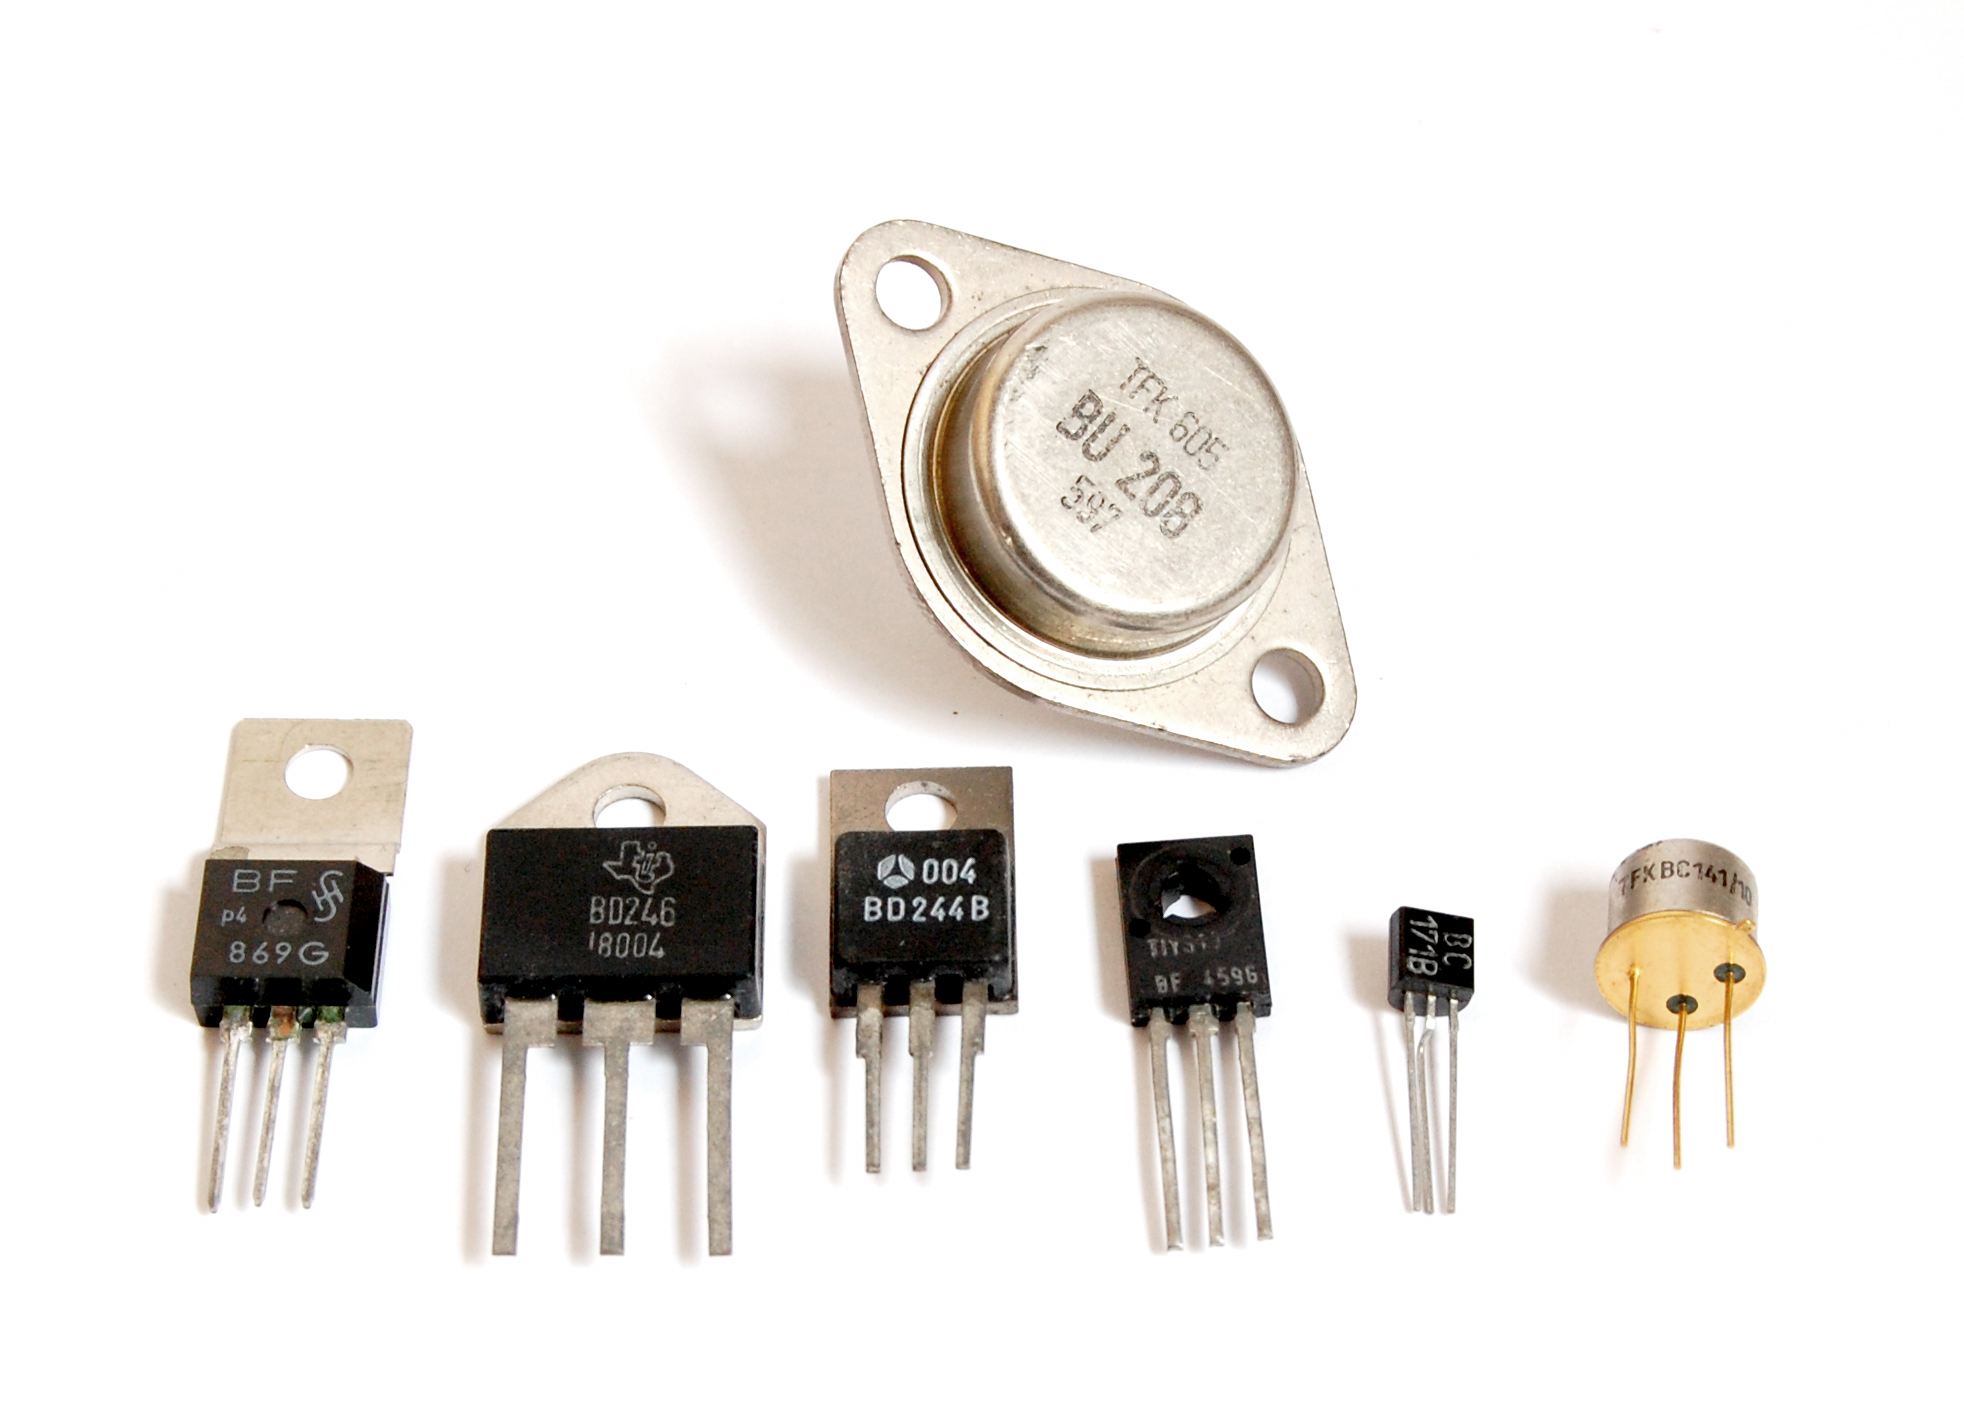
\includegraphics[scale=0.4]{Transistor/Bilder/Transistors-white.jpg}
 \vspace{-6cm}
\end{wrapfigure}

\section*{Theorie- und Prüfungsfragen}

\begin{enumerate}
\itemsep1pt\parskip0pt\parsep0pt
\item[1] Skizziere die Schaltzeichen eines NPN- und eines PNP-Transistors. Beschrifte  entsprechend die Anschlüsse.
\end{enumerate}

\loesung{
\begin{figure}[H]
\centering
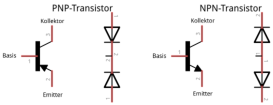
\includegraphics[scale=3]{Transistor/Bilder/PNP_NPN.pdf}
\caption{1 und 2 - NPN- und PNP-Transistor}
\end{figure}
}

\mucho{2}{TC601}
{Was versteht man unter Stromverstärkung beim Transistor?}%Frage
{Mit einem geringen Strom (Basisstrom) wird ein großer Strom (Kollektorstrom) gesteuert.}%A
{Mit einem geringen Strom (Emitterstrom) wird ein großer Strom (Kollektorstrom) gesteuert.}%B
{Mit einem geringen Strom (Emitterstrom) wird ein großer Strom (Basisstrom) gesteuert.}%C
{Mit einem geringen Strom (Kollektorstrom) wird ein großer Strom (Emitterstrom) gesteuert.}%D
{A}%Lösung

\begin{enumerate} 
\itemsep1pt\parskip0pt\parsep0pt
\item[3] \emph{\textbf{TC605}} Welche Kollektorspannungen haben NPN- und PNP-Transistoren?
	\begin{enumerate}
	\itemsep1pt\parskip0pt\parsep0pt
		\item[A] NPN- und PNP-Transistoren benötigen negative Kollektorspannungen.
		\item[B] PNP-Transistoren benötigen positive, NPN-Transistoren negative Kollektorspannung.
		\item[C] PNP- und NPN-Transistoren benötigen positive Kollektorspannungen.
		\item[D] NPN-Transistoren benötigen positive, PNP-Transistoren negative Kollektorspannungen.
		\loesung{Lösung D}
	\end{enumerate}
\end{enumerate}

\begin{enumerate} 
\item[4] \emph{\textbf{TC602}}  Das Verhältnis von Kollektorstrom zum Basisstrom eines Transistors liegt üblicherweise im Bereich von
	\begin{enumerate}
	\itemsep1pt\parskip0pt\parsep0pt
		\item[A] 1 zu 50 bis 1 zu 100.
		\item[B] 10 zu 1 bis 900 zu 1.
		\item[C] 1000 zu 1 bis 5000 zu 1.
		\item[D] 1 zu 100 bis 1 zu 500.
		\loesung{Lösung B}
	\end{enumerate}
\end{enumerate}

\mucho{5}{TC609}
{Ein bipolarer Transistor ist}%Frage
{spannungsgesteuert.}%A
{thermisch gesteuert.}%B
{ein Gleichspannungsverstärker.}%C
{stromgesteuert.}%D
{D}%Lösung

\mucho{6}{TC611}
{Wie erfolgt die Steuerung des Stroms im Feldeffekttransistor (FET)?}%Frage
{Die Gatespannung ist allein verantwortlich für den Drainstrom.}%A
{Die Gatespannung steuert den Widerstand des Kanals zwischen Source und Drain.}%B
{Der Gatestrom ist allein verantwortlich für den Drainstrom.}%C
{Der Gatestrom steuert den Widerstand des Kanals zwischen Source und Drain.}%D
{B}%Lösung

\mucho{7}{TC612}
{Wie bezeichnet man die Anschlüsse des folgenden Transistors?\\ 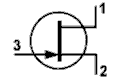
\includegraphics[scale=0.5]{Transistor/Bilder/TC612.png}}%Frage
{1 Drain, 2 Source, 3 Gate.}%A
{1 Source, 2 Drain, 3 Gate.}%B
{1 Anode,  2 Katode, 3 Gate.}%C
{1 Kollektor, 2 Emitter, 3 Basis.}%D
{A}%Lösung

\mucho{8}{TD401}
{In welcher der folgenden Zeilen werden nur Verstärker-Bauelemente genannt?}%Frage
{Transistor, Halbleiterdiode, Operationsverstärker, Röhre}%A
{Transistor, MOSFET, Operationsverstärker, Röhre}%B
{Transistor, Varicap-Diode, Operationsverstärker, Röhre}%C
{Transistor, MOSFET, Halbleiterdiode, Röhre}%D
{B}%Lösung

\mucho{9}{TD402}
{Was versteht man in der Elektronik unter Verstärkung? Man spricht von Verstärkung, wenn ...}%Frage
{das Eingangssignal gegenüber dem Ausgangssignal in der Leistung größer ist.}%A
{z.B. beim Transformator die Ausgangsspannung größer ist als die Eingangsspannung.}%B
{das Ausgangssignal gegenüber dem Eingangssignal in der Leistung größer ist.}%C
{das Eingangssignal gegenüber dem Ausgangssignal in der Spannung größer ist.}%D
{C}%Lösung

\mucho{10}{TD403}
{Was ist ein Operationsverstärker? Operationsverstärker sind ...}%Frage
{Gleichstrom gekoppelte Verstärker mit sehr hohem Verstärkungsfaktor und großer Linearität.}%A
{Wechselstrom gekoppelte Verstärker mit niedrigem Eingangswiderstand und großer Linearität.}%B
{in Empfängerstufen eingebaute Analogverstärker mit sehr niedrigem Verstärkungsfaktor aber großer Linearität.}%C
{digitale Schaltkreise mit hohem Verstärkungsfaktor.}%D
{A}%Lösung

\mucho{11}{TD404}
{ Ein IC (integrated circuit) ist...}%Frage
{eine aus vielen einzelnen Bauteilen aufgebaute Schaltung auf einer Platine.}%A
{eine miniaturisierte, aus SMD-Bauteilen aufgebaute Schaltung.}%B
{eine Zusammenschaltung verschiedener Baugruppen zu einer Funktionseinheit.}%C
{eine komplexe Schaltung auf einem Halbleiterkristallplättchen.}%D
{D}%Lösung

\mucho{12}{TD405}
{Worauf beruht die Verstärkerwirkung von Elektronenröhren?}%Frage
{Die Anodenspannung steuert das magnetische Feld an der Anode und damit den Anodenstrom.}%A
{Das von der Gitterspannung hervorgerufene elektrische Feld steuert den Anodenstrom.}%B
{Die Heizspannung steuert das elektrische Feld an der Kathode und damit den Anodenstrom.}%C
{Die Katodenvorspannung steuert das magnetische Feld an der Katode und damit den Gitterstrom.}%D
{B}%Lösung

\newpage

\section*{Praktische Anwendung}

\loesung{In diesem Kapitel geht es um grundlegende Transistorschaltungen. Bei
der Gruppenzusammensetzung von vornherein darauf achten, dass in jeder Gruppe
mind. eine Person mit Löterfahrung zu haben -- solche Leute hat man immer dabei.}

\subsection*{Transistorschaltung 01 - Der Bipolar-Transistor als Schalter}

\begin{enumerate}
\itemsep1pt\parskip0pt\parsep0pt
\item Schaut auch den gegebenen Transistor als Bauteil an. Welche Bezeichnung
  hat er und um welchen Transistortyp handelt es sich? \loesung{BC547C,
    NPN-Bipolartransistor}
\item Ordnet mit Hilfe des Datenblattes die Bezeichnungen der einzelnen Beinchen
  zu. \loesung{CBE $\rightarrow$ Kollektor, Basis und Emitter}
\item Verwendet den Komponententester des Multimeters. Was zeigt dieser an?
  \loesung{Stromverstärkungsfaktor des Transistors, $\beta = h_{FE} \approx 600$}
\item Baut die Transistor-Schaltung aus Abbildung \ref{s01} auf.
\item Legt die Versorgungsspannung an die Schaltung an.
\item Entfernt unter Last die Leuchtdiode 1. Welche Auswirkungen hat das auf die Schaltung und warum?
\end{enumerate}

\begin{figure}[H]
	\centering
	\subfigure[Schaltplan]{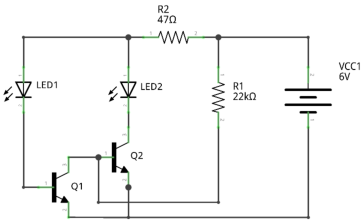
\includegraphics[scale=1.4]{Transistor/Schaltungen/NotBeleuchtung_Schaltplan.pdf}}
	\subfigure[Mögliche Breadboard-Ansicht]{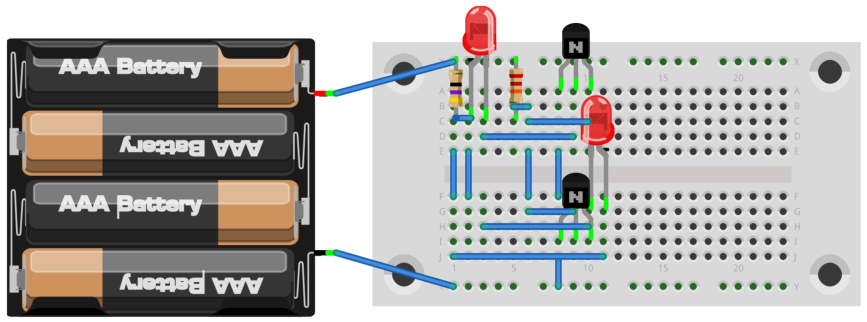
\includegraphics[scale=1]{Transistor/Schaltungen/NotBeleuchtung_Steckplatine.pdf}}
	\caption{Transistorschaltung 01 - Der Bipolar-Transistor als Schalter}
	\label{s01}
\end{figure}

%----------------------------------------------

\subsection*{Transistorschaltung 02 - Der Bipolar-Transistor als Sensor}

\begin{enumerate}
    \itemsep1pt\parskip0pt\parsep0pt
    \item Baut die Transistor-Schaltung aus Abbildung \ref{s02} auf.
    \item Legt die Versorgungsspannung an die Schaltung an.
    \item Berührt die Basis des Transistors Q1 mit dem Finger. Was passiert und warum?
    \item \textbf{Zusatz:} Ersetze die LED durch einen Lautsprecher? Was passiert und warum?
\end{enumerate}

\begin{figure}[H]
	\centering
	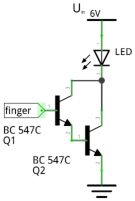
\includegraphics[scale=1.6]{Transistor/Schaltungen/NPN_Sensor.pdf}
	\caption{Transistorschaltung 02 - Der Bipolar-Transistor als Sensor}
	\label{s02}
\end{figure}

%----------------------------------------------

\subsection*{Transistorschaltung 03 - Der Bipolar-Transistor als Verstärker}

\begin{enumerate}
    \itemsep1pt\parskip0pt\parsep0pt
    \item Baut die Transistor-Schaltung aus Abbildung \ref{s03} auf.
    \item Legt die Versorgungsspannung an die Schaltung an.
    \item Legt ein Audiosignal an den Eingang der Schaltung an. Was passiert und warum?
\end{enumerate}

\begin{figure}[H]
	\centering
	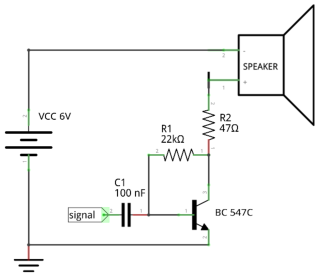
\includegraphics[scale=1.6]{Transistor/Schaltungen/NPN_Verstaerker.pdf}
	\caption{Transistorschaltung 03 - Der Bipolar-Transistor als Verstärker}
	\label{s03}
\end{figure}

%----------------------------------------------

\subsection{Die Lizenz zum Löten}

Übertragt die letzte Schaltung auf eine Lochrasterplatine (ca. $5~x~2.5 cm$).
Den Stecker zur Spannungsversorgung könnt ihr direkt auflöten. Für den Anschluss
der Lautsprecher verwendet eine kleine Buchsenleiste.
